
\chapter{Milestones and Timeline}
\label{ch:timeline}
In this chapter, I describe my progress-to-date, provide a full list of milestones, and present two corresponding timelines for my PhD program.
\autoref{tab:timeline:milestones} shows all dissertation milestones and their current status.
\autoref{fig:timeline:overview} presents a complete, but brief, overview of the entire PhD.
\autoref{fig:timeline:zoom} presents a focused timeline of the remaining plans.


\newcommand{\MilestoneComplete}{ \textcolor[rgb]{0,0.4,0} {Complete}}
\newcommand{\MilestonePublished}[1]{ \textcolor[rgb]{0,0.4,0} {Published: #1}}

\newcommand{\MilestoneScheduled}{ \textcolor[rgb]{0.5,0.6,0.5} {Scheduled}}
\newcommand{\MilestoneAccepted}{ \textcolor[rgb]{0.5,0.6,0.5} {Accepted}}

\newcommand{\MilestoneInReview}{ \textcolor[rgb]{0.6,0.6,0.3} {In Review}}
I
\newcommand{\MilestoneInProgress}{ \textcolor[rgb]{0,0,0.6} {In Progress}}

\newcommand{\MilestonePlanned}{ \textcolor[rgb]{0.7,0.7,0.7} {Planned}}

\newcommand{\MilestoneSideProject}{ \emph{Side Project:} }

% Requires the booktabs if the memoir class is not being used
\begin{table}[htbp]
   \centering
   \begin{tabular}{@{} lllll @{}} % Column formatting, @{} suppresses leading/trailing space
      \toprule
      \textbf{Date} & & \textbf{Component} & \textbf{Milestone} & \textbf{Status} \\
      \midrule
     	2013 & Sept
      	& Haptic Instrument
	& Tool
	& \MilestoneComplete
	\\
	
	
      	& &
	& Paper \& Demo
	& \MilestonePublished{HAPTICS'14}
	\\
	
	2014 & June
      	& \MilestoneSideProject FeelCraft
	& Paper
	& \MilestonePublished{AsiaHaptics'14}
	\\
	
	 & Sept
      	& Tactile Animation
	& Tool
	& \MilestoneComplete
	\\
	
	
      	& &
	& Paper
	& \MilestoneInReview
	\\
	
	& Oct
    	& \MilestoneSideProject FeelCraft
	& Demo
	& \MilestonePublished{UIST'14}
	\\
	
	
	 & Dec
      	& PhD Requirements
	& Course Requirement
	& \MilestoneComplete
	\\
	
	2015 & Jan
      	&  \MilestoneSideProject Feel Messenger
	& Short Paper
	& \MilestonePublished{CHI'15}
	\\
      
      	 & \bf June
      	& \bf PhD Requirements
	& \bf Proposal Defence
	& \MilestoneScheduled
	\\
	
	
      	&  
	& HaXD Workshop
	& Workshop
	& \MilestoneAccepted
	\\
	
	&
      	&  \MilestoneSideProject Feel Messenger
	& Demo
	& \MilestoneAccepted
	\\
	
		
	&
      	&  \MilestoneSideProject RoughSketch
	& Demo
	& \MilestoneAccepted
	\\
	
	& Sept
      	&  Design Gallery
	& Tool
	& \MilestoneInProgress
	\\
	
	
	&
      	&  \MilestoneSideProject CuddleBit
	& Paper
	& \MilestoneInProgress
	\\
	
	&
      	&  \MilestoneSideProject HapTurk
	& Paper
	& \MilestoneInProgress
	\\
	
	&
      	&  \MilestoneSideProject CyberHap
	& Paper
	& \MilestoneInProgress
	\\
	
	& Nov
     	&  Design Gallery
	& Paper
	& \MilestonePlanned %\footnote{I currently have a stretch goal to attempt a paper in Sept 2015, but given the number of side projects I assume it will be delayed.}
	\\
	
	2016 & Jan
      	&  HaXD Workshop
	& Short Paper
	& \MilestonePlanned
	\\
	
	 & March
      	&  PhD Requirements
	& Dissertation Draft
	& \MilestonePlanned
	\\
	
	 & May
      	&  HaXD Theory
	& Paper
	& \MilestonePlanned
	\\

	 & July
      	&  PhD Requirements
	& Final Defence
	& \MilestonePlanned
	\\
	
	
      
      \bottomrule
   \end{tabular}
   \caption{PhD milestones and current status.}
   \label{tab:timeline:milestones}
\end{table}


\textbf{Progress on in-depth case-studies:}
I have currently finished and presented the work described in Case Study 1 (The Haptic Instrument, \autoref{ch:hapticinstrument}) at Haptics Symposium 2014 \cite{Schneider2014} and a CHI 2014 workshop \cite{Schneider2014b}.
I have also finished and written up the work described in Case Study 2 (Tactile Animation, \autoref{ch:hapticanimation}); a paper has been submitted to UIST 2015.
I have already reviewed the literature, prototyped algorithms, and started building my study platform for Case Study 3 (Design Gallery, \autoref{ch:hapticexamples}), with plans to finish the study platform (Phase I) and begin the design study (Phase II) in summer 2015, and submit a paper to a top-tier conference in fall 2015.

\textbf{Progress on side-projects:}
I have also began all side projects.
The FeelCraft project, on software architecture for adding customized vibrotactile (VT) effects to video games, has already been written and presented at Asia Haptics 2014 \cite{SchneiderAsiaHaptics2014} and as a UIST 2014 demo.
The Feel Messenger project, on sending customized VT sensations via commercial smartphones, has had a work-in-progress published at CHI 2015 \cite{Israr2015} and a demo accepted to World Haptics 2015.
Other side projects are currently underway as projects led by summer students in 2015. Paper submissions are planned in fall 2015, on which I will participate as an author in a supervisory role; the RoughSketch project will result in a demo at World Haptics 2015, presented by summer students.

\textbf{Progress on theory development:}
%Grounded data from haptic experts is currently planned.
The HaXD'15 workshop on Haptic Experience design is planned, accepted, and scheduled for World Haptics in June 2015; afterwards, a small retrospective piece is planned in winter 2016 (either on its own or as part of a larger submission).
The data from haptic designers has already been collected by UBC Alumnus Colin Swindells; I plan to digest and analyze those interviews in winter 2016, and submit findings for my preliminary theory to a conference or journal in 2016 (depending on my dissertation submission timeline).


\begin{figure}[htbp] %  figure placement: here, top, bottom, or page
   \centering
   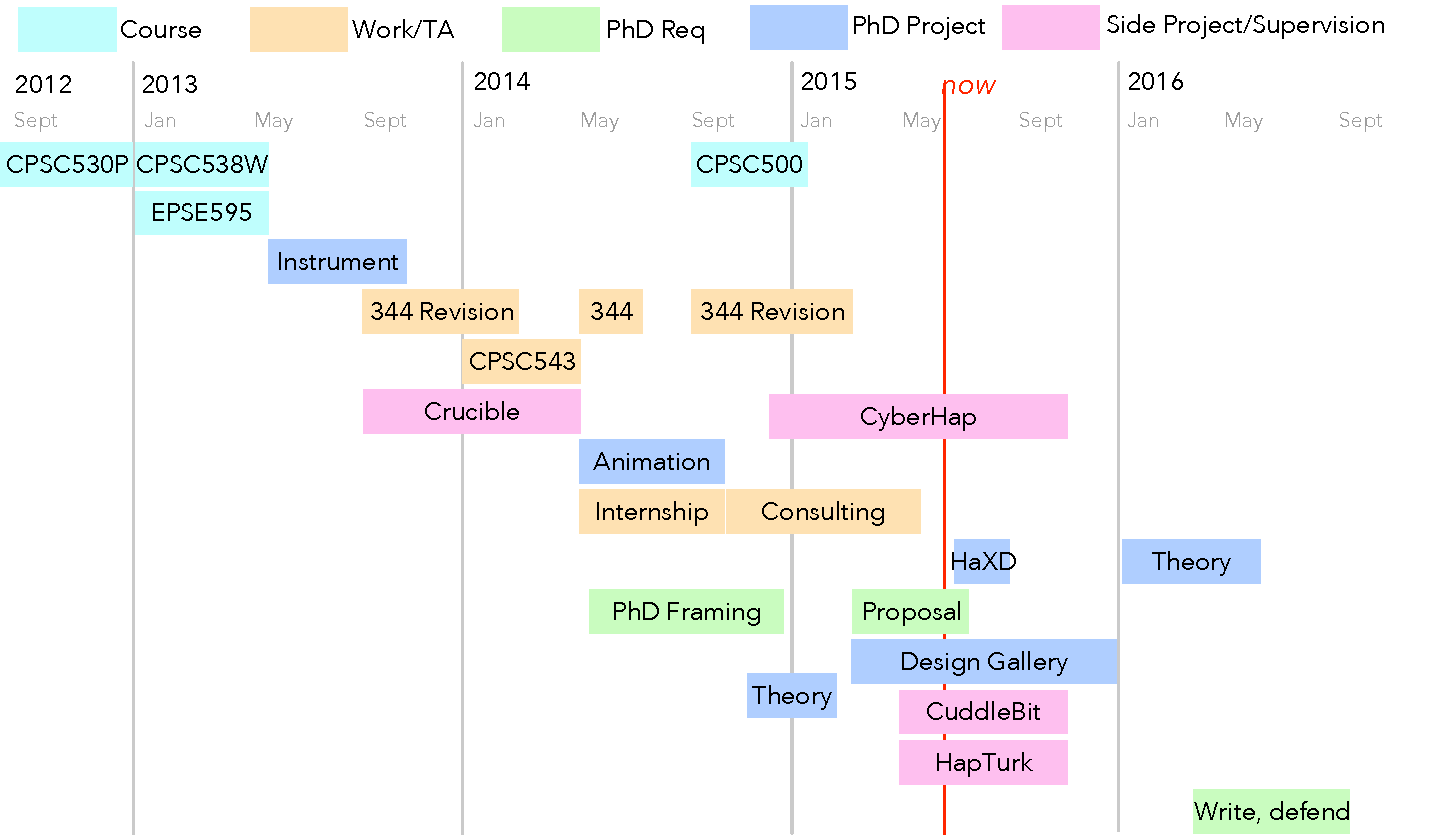
\includegraphics[width=\textwidth]{PhDTimelineOverview-2015-05-28} 
   \caption{Overview of PhD from start (September 2012) to intended finish (August 2016).}
   \label{fig:timeline:overview}
\end{figure}

\begin{figure}[htbp] %  figure placement: here, top, bottom, or page
   \centering
   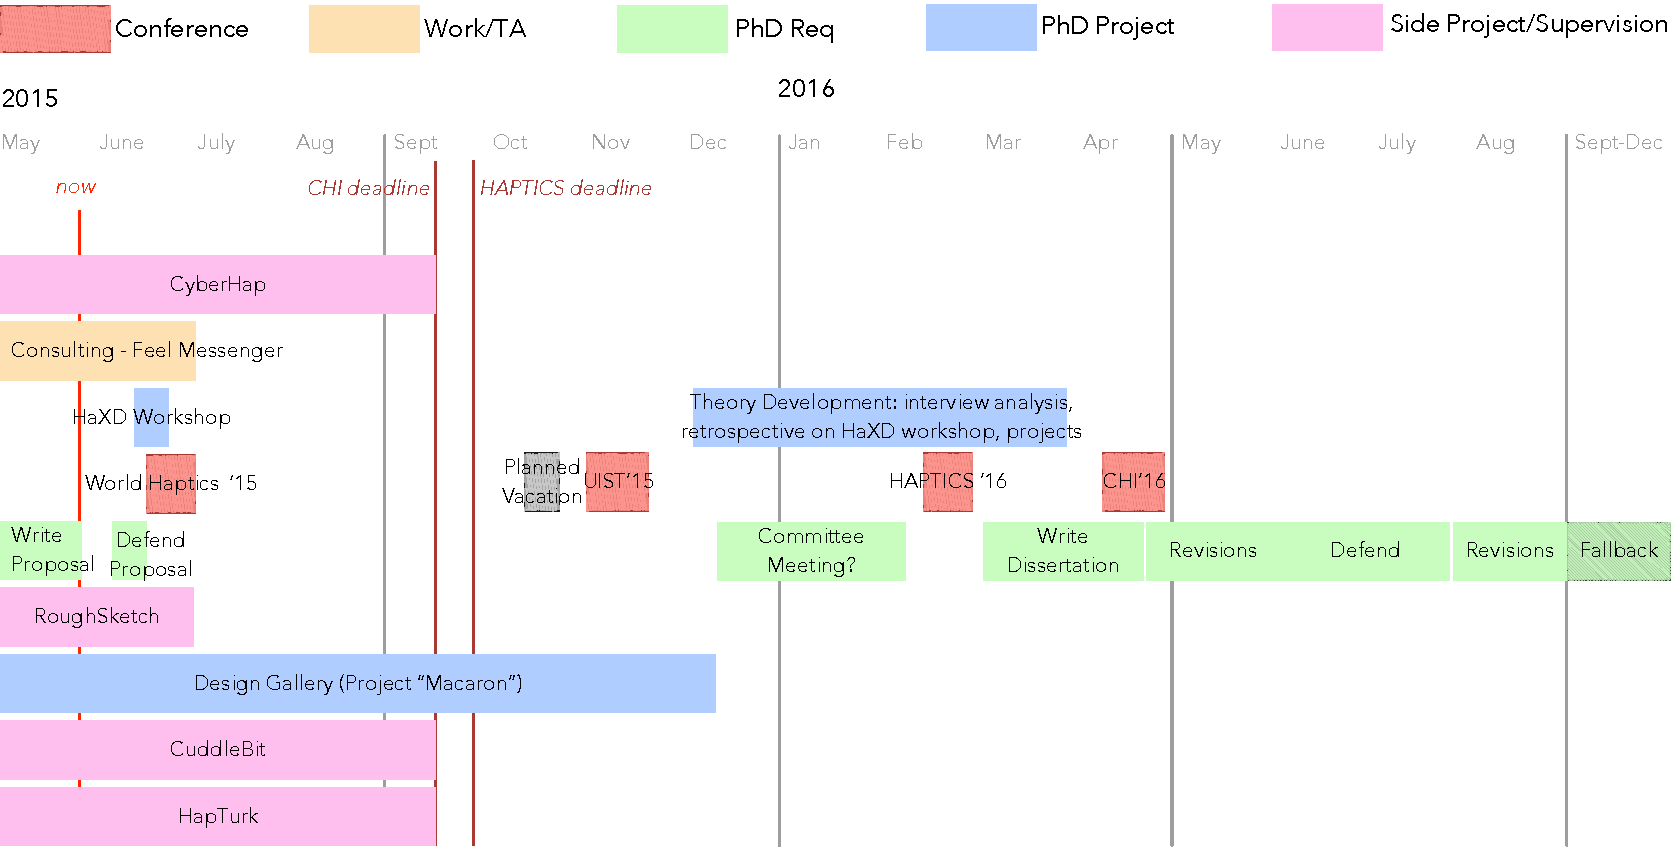
\includegraphics[width=\textwidth]{PhDTimelineZoom-2015-05-28} 
   \caption{Detailed timeline of remaining plans, from May 2015 to intended finish (August 2016). Note that several projects are targetting the CHI'16 deadline, but could also be submitted to the coinciding HAPTICS deadline based on fit.}
   \label{fig:timeline:zoom}
\end{figure}

\endinput
